%\part{O Bitcoin Client}
\chapter{Quem faz as regras?}
\label{ch:capitulo8}

Agora temos um sistema distribuído funcional para acompanhar e transferir valor.
Vamos revisar o que criamos até agora:

\begin{samepage}
\begin{enumerate}
\item Um livro-razão distribuído, uma cópia que é mantida por todos os participantes;
\item Um sistema de loteria baseado em Prova de Trabalho e ajustes de dificuldade para manter a rede segura e o cronograma de emissão consistente;
\item Um sistema de consenso que garante que cada participante possa validar todo o histórico da blockchain para si, usando um software de código aberto chamado Bitcoin Client;
\item Um sistema de identidade usando assinaturas digitais que permite a criação arbitrária de caixas de correio semelhantes a contas que podem receber bitcoins sem uma autoridade central.
\end{enumerate}
\end{samepage}

Agora é hora de enfrentar uma das coisas mais interessantes e contra-intuitivas do Bitcoin: De onde vêm as regras, como são aplicadas e como elas podem ser modificado ao longo do tempo.

\section*{O software do Bitcoin}


Ao longo dos capítulos anteriores, presumimos que todos na rede estavam validando as mesmas regras: ou seja, estão rejeitando gastos duplos, garantindo que cada bloco contenha a quantidade adequada de Prova de Trabalho, que cada bloco aponte para o bloco anterior da blockchain atual e que cada transação contida no bloco esta devidamente assinada pelo proprietário daquele endereço, entre um monte de outras coisas com as quais as pessoas concordaram ao longo do tempo.

Também dissemos que o Bitcoin é um software de código aberto. 
O código aberto significa que qualquer pessoa pode ler seu código e também que qualquer pessoa pode atualizar sua própria cópia com o código que quiser. 
Como as mudanças chegam ao Bitcoin?

O Bitcoin é um \textit{protocolo}.
Em software de computador, este termo se refere a um conjunto de regras que o software segue.
No entanto, contanto que você siga o conjunto de regras que todos estão seguindo, você é livre para modificar seu software como desejar.
Quando dizemos que as pessoas “executam nodes de Bitcoin”, o que realmente queremos dizer é que elas executam um software que se comunica usando o protocolo Bitcoin.
Este software pode conversar com outros nodes Bitcoin, transmitir transações e blocos para eles, descobrir outros nodes para fazer se conectar e assim por diante.

Os detalhes reais de como o software é implementado dependem de qualquer pessoa que o execute.
Na verdade, existem muitas implementações do protocolo Bitcoin.
O mais popular deles é chamado Bitcoin Core e é a extensão do trabalho lançado pela primeira vez por Satoshi Nakamoto.

Existem outros clientes também, alguns até mesmo escritos em outras linguagens de computador e mantidos por pessoas diferentes. 
Como o consenso em Bitcoin é crítico, o que significa que todos os nodes devem concordar sobre quais blocos são ou não válidos, a grande maioria dos nodes executa o mesmo software (Bitcoin Core) para evitar quaisquer bugs acidentais que podem fazer com que alguns nodes discordem sobre o que é válido ou não.
Na verdade não existe uma lista de especificações completas e escritas do protocolo bitcoin, então a melhor aposta para implementar um novo software do bitcoin é ler o código original e ter certeza que não desviaste do que ele faz, mesmo com bugs.

\section*{Então, quem faz as regras?}

As regras que compõem o Bitcoin são codificadas no cliente Bitcoin Core. Mas quem decide essas regras? Por que dizemos que o Bitcoin é escasso se alguém pode entrar e fazer uma modificação no software que muda o limite de 21 milhões de bitcoins para 42 milhões?

Sendo um sistema distribuído, todos os nodes deste sistema devem concordar com as regras.
Se você for um minerador e decidir mudar o software para conceder a você o dobro de Bitcoins que lhe é permitido pela configuração atual de recompensa por bloco, então, quando você minerar seu bloco, todos os outros nodes da rede rejeitarão seu bloco. 
Fazer uma mudança nas regras é extremamente difícil porque existem milhares de nodes distribuídos em todo o mundo, cada um aplicando as regras do Bitcoin.

O modelo de governança do Bitcoin é contra-intuitivo, especialmente para aquelas pessoas que vivem em uma democracia ocidental.
Estamos acostumados à governança pelo voto - a maioria das pessoas pode decidir fazer algo, aprovar uma lei e impor sua vontade à minoria.
Mas o sistema de governo do Bitcoin está muito mais próximo de uma anarquia do que da democracia. 

Cada Pessoa que aceita pagamentos em Bitcoin decide por ela mesma o que ela considera ser o Bitcoin.
Se alguém roda um software que diz que à 21 milhões de bitcoins, e você tenta enviar a eles bitcoins produzidos pelo seu software pirata que desafia esse limite, suas moedas aparentarão ser falsificadas para eles logo serão rejeitadas.

Vamos dar uma olhada nos entes que compõe este sistema:

\textbf{Node}: Cada participante da rede Bitcoin executa um node.
Eles escolhem qual software executar.
Embora a maioria das pessoas execute o Bitcoin Core, a principal implementação do protocolo bitcoin que foi iniciado pelo Satoshi e agora é desenvolvido por centenas de desenvolvedores independentes e diversas empresas ao redor do mundo.
Se essa implementação do software se tornar malicioso e tentar introduzir algo como inflação, ninguém o executará. 
Exemplos de nodes incluem aqueles executados por qualquer pessoa que aceite Bitcoin - comerciantes, exchanges, empresas que oferecem carteiras e pessoas comuns que usam o Bitcoin para qualquer propósito que desejem.

\textbf{Mineradores}: Alguns nodes também mineram bitcoins, gravando transições e tornando muito custoso para alguém adulterar o livro-razão.
%Isso significa que eles gastam eletricidade para ganhar direitos de escrever no livro-razão do Bitcoin.
%Isso fornece a segurança da rede, tornando muito caro para alguém adulterar o livro-razão.
Se os mineradores são os únicos que escrevem nele, pode ser tentador considerá-los os criadores das regras, mas não são. 
Eles estão simplesmente seguindo as regras definidas pelos nodes que aceitam os bitcoins.
Se os mineradores começarem a produzir blocos que contenham recompensa extra, eles não serão aceitos por outros nodes, tornando essas moedas inúteis. Assim, cada usuário executando um node está participando de uma governança anárquica - eles estão escolhendo quais regras as moedas que eles consideram Bitcoin devem seguir, e qualquer violação é rejeitada imediatamente.

\textbf{Usuários/investidores}: Os usuários são as pessoas que compram e vendem a moeda bitcoin e bem como também rodar nodes.
Muitos usuários atualmente não executam seus próprios nodes, mas dependem de um node hospedado pelo provedor da carteira, onde atua como uma espécie de proxy para os desejos e vontades do usuário. 
Os usuários decidem o valor da moeda no livre mercado através da oferta e demanda.
Mesmo que os mineradores e exchanges %a maioria dos nodes econômicos do sistema 
conspirassem e introduzissem algum tipo de mudança radical, como a inflação, os usuários provavelmente se livrariam da moeda que seguisse essas regras, baixando o preço e colocando as empresas que aceitaram essa regra à falência. 
Uma minoria intolerante de usuários sempre poderia manter sua própria versão do Bitcoin viva, que ainda seguisse as regras originais
%, mesmo se o Bitcoin se transformasse em algo de que não gostassem.

\textbf{Desenvolvedores}: O software do Bitcoin Core é o maior projeto do Bitcoin Client que existe.
Ele atraiu um rico ecossistema de centenas dos melhores desenvolvedores e empresas de criptografia.
O projeto central é muito conservador, pois o software alimenta uma rede que agora protege centenas de bilhões de dólares.
Cada ideia de mudança passa por um processo chamado \textit{Bitcoin improvement proposal}\footnote{leia mais sobre o desenvolvimento do Bitcoin Core é gerido em \textit{Who controls Bitcoin Core?} por Jameson Loop:https://medium.com/@lopp/who-controls-bitcoin-core-c55c0af91b8a} e qualquer modificação no código é cuidadosamente revisada por pares. %https://blog.lopp.net/who-controls-bitcoin-core-/} 
 O processo de propostas e revisão de código é feito de maneira  totalmente aberta. 
 Qualquer pessoa pode participar, comentar ou enviar o código. 
 Se os desenvolvedores se tornarem mal intencionados e introduzirem algo que ninguém deseja executar, os usuários simplesmente executarão softwares diferentes. 
 Talvez versões mais antigas, ou começarão a desenvolver algo novo. 
 Por causa disso, os desenvolvedores principais devem desenvolver mudanças que os usuários geralmente desejam, ou arriscam perder seu status de implementação de referência se ninguém quiser executá-la.

\section*{Forks Modificadores de regras}
%\paragraph{}

%nao possui na minha versao
%Deixamos o tópico mais complexo do Bitcoin para o final.

%modificado
Esperamos que agora você tenha um boa ideia sobre como o software Bitcoin impõe as regras que as pessoas concordaram e como as pessoas podem decidir qual software executar para aplicar as regras em que acreditam.

Também falamos que os mineradores decidem as regras que seguirão ao produzir blocos e que devem minerar o tipo de blocos que os usuários desejam, ou arriscar que seus blocos não sejam aceitos e, assim, perder a recompensa da mineração.

Finalmente, sabemos que o software do Bitcoin aceitará a mais longa cadeia de prova cumulativa de trabalho como sendo a única verdadeira rede, e que forks (ou bifurcações em português), às vezes, ocorrem naturalmente devido à mineração dos mineradores usando as cadeias desatualizadas.

%adicionado
Devido a vasta diversidade de participantes na rede, as regras do Bitcoin estão quase que escritas em pedra desde o começo. As únicas melhorias que foram executadas no bitcoin ate então foram feitas de maneira retro compatível, preservando as regras de consenso para nodes que não aplicaram as melhorias.

%modificado
Agora vamos falar sobre como regras podem ser modificadas.
Um fork intencional é quando alguns usuários e/ou mineradores decidem que não concordam com as regras atuais do Bitcoin e que precisam mudar as regras. 
Existem dois tipos de forks, que mudam as regras que foram encontrados na natureza: soft forks, que são compatíveis com versões anteriores, e hard forks, que não são compatíveis com versões anteriores.
Vamos ver como isso ocorre na teoria e, em seguida, ver alguns exemplos históricos\footnote{A historia completa de forks modificadores de regras podem ser analisados aqui \url{https://blog.bitmex.com/bitcoins-consensus-forks/}}.

%MInha versao nao tem essas divisas
% \paragraph{Soft Forks}
% \paragraph{}

%modificado
Um soft fork é uma mudança retro compatível com as regras de consenso do Bitcoin que aperta as regras.
Isso significa que se você executar um node antigo que não foi atualizado para as novas regras, ele ainda verá os blocos produzidos sob as novas regras como válidos. 
Vejamos um exemplo para deixar claro:
%Para um node atualizado com o novo software soft fork, todos os blocos que eram anteriormente inválidos permanecem inválidos, mas alguns blocos válidos agora são considerados inválidos. (removido)

%modificado
Em 12 de setembro de 2010, uma nova regra foi introduzida no software: Os blocos devem ter no máximo 1 MB de tamanho. 
Esta regra foi introduzida para resolver problemas de spam na blockchain.
Antes dessa regra, todos os blocos de qualquer tamanho eram válidos.
Com a nova regra, apenas blocos menores eram válidos, logo as regras ficaram mais rígidas.
Se você estava executando um node antigo e não o atualizou, os blocos menores ainda eram válidos de acordo com suas regras, então você não foi afetado.

Um soft-fork é uma maneira de atualizar o sistema sem interrupções porque permite que os operadores dos nodes atualizem para o novo software lentamente ao longo do tempo, de forma voluntária.
Se eles não fizerem a atualização, eles ainda serão capazes de processar todos os blocos que chegam como sempre fizeram.
Apenas os  mineradores que produzem os blocos precisam se atualizar para começar a produzir blocos usando as novas regras.
Depois que os mineradores atualizaram para o novo fork de 1 MB, todos os blocos daquele ponto em diante tinham no máximo 1 MB de tamanho.
Os usuários que executam versões antigas do software não precisavam saber disso.


% \paragraph{Hard Forks}
% \paragraph{}

%Um hard fork é o oposto de um soft fork.
No caso de um hard fork, uma alteração não compatível com versões anteriores é introduzida.
Um hard fork é uma expansão do banco de regras na qual os blocos que eram originalmente inválidos agora são considerados válidos.
Os nodes antigos que não foram atualizados não serão capazes de processar os blocos produzidos sob as novas regras. 
Assim, eles ficarão presos na blockchain antiga, a menos que façam a atualização. 

%removido
%Um exemplo de hard fork seria aquele que alterasse o tamanho do bloco de 1 MB para algo maior, pois os blocos seriam inválidos de acordo com as regras antigas.

%modificado
Hard forks com concordância quase unânime de todos os nodes da rede não causaria problemas. 
Cada node seria atualizado imediatamente para as novas regras. 
Se alguns retardatários fossem deixados para trás, eles não obteriam novas atualizações de bloco e teoricamente notariam que seu software parou de funcionar e seriam forçados a atualizá-los.

Na prática, os hard forks nunca são feitos de maneira suave.
Em um sistema anárquico verdadeiramente descentralizado, você não pode coagir todos a mudarem para as novas regras.
Em agosto de 2017, algumas pessoas que não estavam felizes com o progresso da rede Bitcoin em relação a pagamentos baratos decidiram que queriam fazer um fork para criar uma rede com blocos maiores. 
Como o Bitcoin tinha uma regra sobre os blocos não ultrapassarem 1 MB, devido a um soft fork ocorrido em 2010. 
Essas pessoas queriam criar uma nova cadeia com blocos maiores.
Este fork ficou conhecido como Bitcoin Cash.

%modificado
Um hard fork fora do consenso como Bitcoin Cash, que não é seguido por todos os mineradores e nodes, cria uma nova blockchain.
Essa blockchain compartilha alguma história com a blockchain original incluindo as UTXO(saldo de conta) existentes ate o ponto da divisão. 
Mas, a partir do ponto de divisão em diante, as moedas criadas no fork não são mais Bitcoin, pois não são aceitas por nenhum node da rede Bitcoin.

%modificado
O assunto o que “é” ou “não é” Bitcoin foi calorosamente debatido no ano seguinte ao fork do Bitcoin Cash.
Houve algumas pessoas em favor do Bitcoin Cash que propuseram uma narrativa de que o Bitcoin deve ser definido pelo que está escrito no white paper original, escrito por Satoshi há dez anos. 
Escolhendo a dedo as palavras específicas no documento para provar seu ponto. 
Mas um sistema baseado em consenso não funciona com apelo a autoridades. 
Funciona pela ação coletiva de muitos indivíduos incluído por optarem que software executar, e que moeda comprar ou vender no mercado livre.

No caso deste fork, as pessoas que executam a grande maioria dos nodes economicamente significativos - ou seja, carteiras, exchanges e comerciantes não queriam trocar seu software por algo suportado por uma equipe de desenvolvimento muito menor e menos experiente e em uma quantidade muito menor de hash. %que sinalizou que eles queriam mudar para essas regras. 
Nem as pessoas achavam que tal “atualização” valesse a pena quando comparado a possibilidade de interrupção do ecossistema. 
O problema com os hard forks é que eles só funcionam quando todos aceitam a troca.
Se houver retardatários, duas moedas são criadas. 
Assim, o Bitcoin permaneceu como sendo o Bitcoin e o Bitcoin Cash tornou-se uma moeda separada.
Como todos que já tinham bitcoin receberam bitcoin Cash livre de custo, muitos apenas venderam a moeda por "dinheiro gratuito" o que empurrou o preço do bitcoin Cash para baixo

Hoje, existem dezenas de outros forks de Bitcoin, como Bitcoin SV(que por se só é um fork do Bitcoin Cash) Bitcoin Gold, Bitcoin Diamond e Bitcoin Private. Todos eles com um pequeno hash protegendo-os, baixo suporte ao desenvolvedor, com atividade na rede quase inexistente e baixa liquidez em exchange.
A sua falta de liquidez faz dessas moedas um ótimo alvo para subidas e quedas manipuladas, que frequentemente levam a subidas meteóricas de preço e iguais quedas espetacularmente devastadoras. 
Muitas foram sujeitas a hacks em suas carteiras, ataques de 51\% e outros desastres. 
Muitos são golpes ou campo de batalha para apostadores. 
A maioria tem um algo grau de centralização em algum aspecto do seu projeto. 
O site \url{forkdrop.io} esta atualmente acompanhando 74 tentativas de Bitcoin.

\begin{figure}
    \centering
    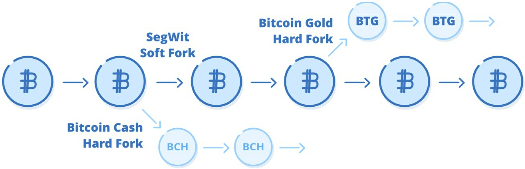
\includegraphics[width = 10cm]{imagens/Capitulo8/capitulo8-forks.png}
    \caption*{\textit{\small Moedas de um soft-fork podem ser enviada a nodes antigos. Um Hard-fork produz um novo retro incompatível UTXOs que não será aceito por nodes antigos}}
\end{figure}


Centenas de moedas semelhantes ao Bitcoin usam código semelhante, mas não compartilham o histórico de saldo da conta do Bitcoin (conjunto UTXO), como Litecoin ou Dogecoin.
Essas não são tipicamente consideradas divisões do Bitcoin embora dividam muito do mesmo código, pois elas não compartilham o histórico de saldo nas carteiras do bitcoin.

Um fork do Bitcoin não impacta sua oferta máxima de 21 milhões de Bitcoins. 
Imagine que você tem as reservas de ouro do mundo em um forte ultra seguro com segurança pesada.
Você construir uma pequena, mal montada cabana e chamar ela de forte lite, protegendo ela com um único segurança.
Podes pintar umas pedras de ouro e colocar elas dentro da cabana.
Quando anunciares ao mundo que você "forkou" o ouro e todos que detêm ouro podem deter a mesma quantia de pedras douradas em sua cabana.

Nos precisamos de muitos mineradores protegendo o bitcoin, tornando ele custoso a ataques de 51\%.  
Um fork do Bitcoin que só possui alguns mineradores, semelhantes a sua cabana mal protegida, é fácil de atacar. 
O código é provavelmente estruturalmente inseguro, construído por uma equipe de desenvolvedores sem experiencia, com péssima revisão por pares, igual a sua cabana. 
Moedas de forks não são aceitas por nodes porque quebram as regras do Bitcoin. 
Da mesma maneira que pessoas que tem testes químicos para o ouro não irão aceitar suas pedras douradas.
O custo de manufaturar as pedras e as moedas do fork é zero visto que deste elas de graça para todos os proprietários de ouro. 
Isso é limita o interesse do mercado em forks do Bitcoin.

Enquanto você considera as milhares de copias do Bitcoin que já foram criadas, e nenhuma os quais possui valor de mercado significativo, pense nesse paradoxo:
Criar forks do Bitcoin é gratuito e fácil. Porem, mudar as regras do Bitcoin ou criar Bitcoin novos é tudo menos fácil. 
A próxima vez que você ouvir alguém com conhecimento limitado sobre o bitcoin perguntar porque o Bitcoin é especial responda com isso.


%modificado
A natureza descentralizadas do ecossistema do Bitcoin cria uma forte preferencia ao modelo atual. 
Mudanças significativas precisam de meses ou anos de muito debates, construções de consenso e revisão por pares para ser implementado.
Isso é algo bom, e algo que almejamos de um sistema que visa ser a moeda do planeta.
Bitcoin é uma dança delicada entre milhares de participantes, todos agindo de forma egoísta e muitas vezes com necessidades concorrentes.
É um sistema anarquista de mercado verdadeiramente livre, sem ninguém em particular no comando.